\documentclass[a4paper, 12pt, finnish]{article}
\usepackage{babel}
\usepackage{afterpage}
\usepackage[utf8]{inputenc}
\usepackage[T1]{fontenc}
\usepackage{amsmath}
\usepackage[margin=0.9in]{geometry}
\geometry{a4paper}
\usepackage{graphicx}
\usepackage{float}
\usepackage{wrapfig}
\usepackage{caption}
\usepackage{eurosym}
\usepackage[section]{placeins}
\usepackage{url}
\usepackage[hidelinks]{hyperref}
\usepackage{hyperref}
\usepackage{subcaption}
\usepackage{lipsum}
\usepackage{changepage}
\usepackage{bookmark}
\usepackage[table,xcdraw]{xcolor}
\usepackage[export]{adjustbox}
\definecolor{grey}{rgb}{0.9,0.9,0.9}
\def\UrlBreaks{\do\/\do-}
\graphicspath{{./figures/}}
\usepackage{titlesec}

\setcounter{secnumdepth}{4}

\titleformat{\paragraph}
{\normalfont\normalsize\bfseries}{\theparagraph}{1em}{}
\titlespacing*{\paragraph}
{0pt}{3.25ex plus 1ex minus .2ex}{1.5ex plus .2ex}

\begin{document}
\begin{titlepage}
	\colorbox{grey}{
		\parbox[t]{0.93\textwidth}{
			\parbox[t]{0.91\textwidth}{
				\raggedleft
				\fontsize{80pt}{80pt}\selectfont
				\vspace{0.7cm}
				\textbf{MX Linux 18\\
				käyttöopas\\}
				\vspace{0.7cm}
			}
		}
	}
	\vfill
	\parbox[t]{0.93\textwidth}{
		\raggedleft
		\large
		{\Large Iiro Aarnio}\\[4pt]
		Projektissa toimiminen\\
		Tampereen seudun ammattiopisto\\[4pt]
		\url{github.com/maysion/mxlinux18}\\
		\hfill\rule{0.2\linewidth}{1pt}
	}
\end{titlepage}
\thispagestyle{empty}
\begin{abstract}
	Tässä käyttöoppaassa perehdytään MX Linux 18 -GNU/Linux-jakelun käyttöönottoon ja käyttöön. Käyttöopas on suunnattu henkilöille, joilla ei ole aiempaa kokemusta Linux-järjestelmistä. Käyttöopas sisältää muun muassa käyttöjärjestelmän asentamisen, ohjelmien hakemisen ja päivittämisen. Opas ei sisällä laitteiston valmistelua.
\end{abstract}

\newpage
\thispagestyle{empty}
\tableofcontents
\newpage
\pagenumbering{arabic}
\setcounter{page}{1}
\newpage

%%% DOC

\section{Mikä on MX Linux 18?}
MX Linux 18 on työpöytäkäyttöön tarkoitettu GNU-käyttöjärjestelmään pohjautuva jakelu. Puhekielessä näistä jakeluista puhutaan usein Linux-käyttöjärjestelminä. Tässä oppaassa käytetään oikeaoppista termiä, GNU/Linux-jakelu.

MX Linux 18 perustuu tunnetumpaan GNU/Linux-jakeluun nimeltä Debian. Sadat eri GNU/Linux-jakelut perustuvat Debian-nimiseen GNU/Linux-jakeluun, sillä se on vakaa ja suhteellisen helposti muokattavissa käyttäjäystävälliseksi.

\subsection{Miten MX Linux 18 eroaa muista käyttöjärjestelmistä?}
MX Linux 18 eroaa monin eri tavoin muista markkinoilla olevista käyttöjärjestelmistä, sillä se pohjautuu GNU-käyttöjärjestelmään ja hyödyntää Linux-ydintä.

Työpöytäkäytössä GNU/Linux-järjestelmien edut ovat huomattavat. Suuri osa GNU/Linux-jakeluista ovat todella kevyitä ja toimivat hyvin vanhemmalla laitteistolla. Markkinoiden suosituimmat käyttöjärjestelmät, Microsoft Windows sekä MacOS, ovat todella raskaita käyttöjärjestelmiä ja vaativat suhteellisen uutta laitteistoa. MX Linux 18 on kevyt ja suunniteltu toimivaksi mahdollisimman monilla erilaisilla laitteistolla.

\section{Livetilaan käynnistäminen}
MX Linux 18 -jakelun käynnistyttyä käynnistysmedialta, avautuu kuvanmukainen valikko. (Kuva \ref{fig:boot})
Painamalla F2-näppäintä, voidaan valita haluttu kieli. Valintaa voi muokata nuolinäppäimillä. (Kuva \ref{fig:lang}) Kieliasetus on hyvä määrittää tässä vaiheessa, sillä se määrittää koko asennusprosessin kielen.

\begin{figure}[htbp]
     \centering
      \begin{minipage}{.5\textwidth}
           \centering
            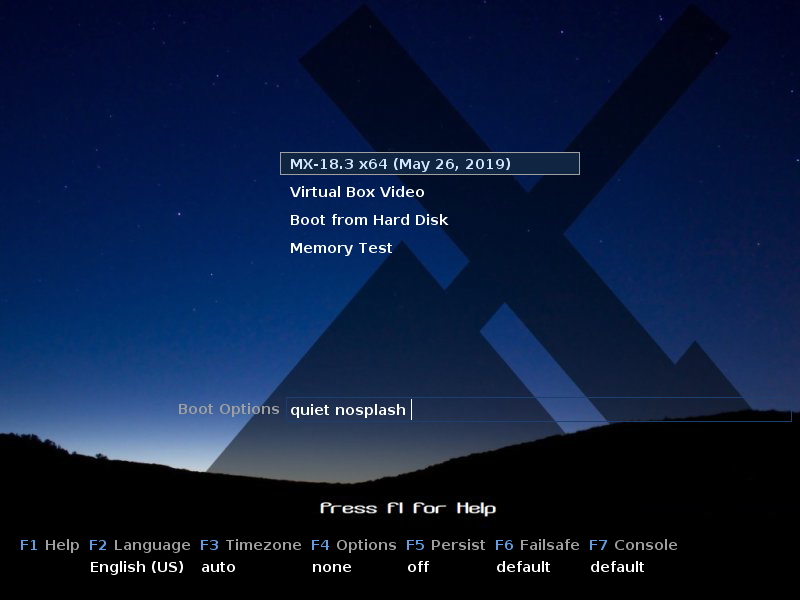
\includegraphics[width=.98\linewidth]{asen/boot}
             \captionof{figure}{Käynnistysvalikko}
              \label{fig:boot}
               \end{minipage}%
               \begin{minipage}{.5\textwidth}
                    \centering
                     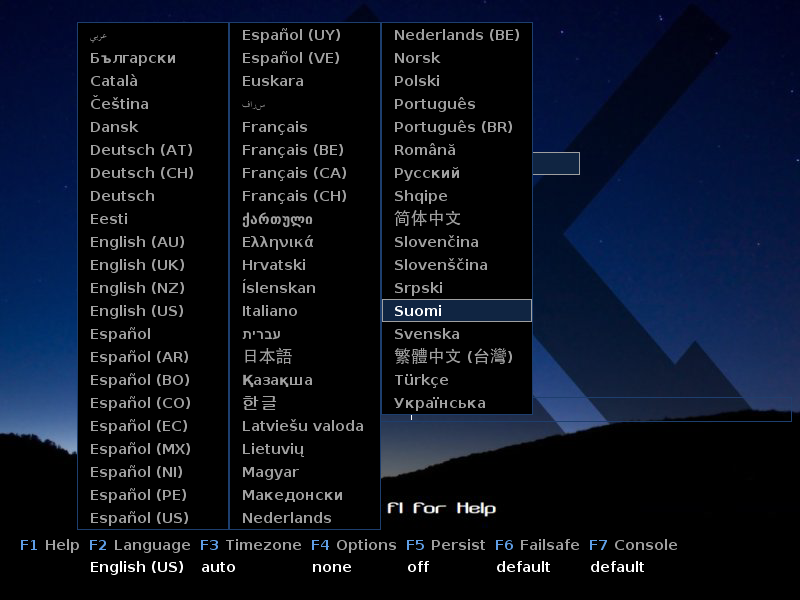
\includegraphics[width=.98\linewidth]{asen/lang}
                      \captionof{figure}{Käynnistysvalikon kieliasetukset}
                       \label{fig:lang}
                        \end{minipage}
                         \end{figure}


Kielen valitsemisen jälkeen jakelun voi käynnistää niin kutsuttuun livetilaan, painamalla Enter-painiketta.

\subsection{Tietoa livetilasta}

Toisin kuin yleisimmät kaupalliset käyttöjärjestelmät, GNU/Linux-jakelut käynnistyvät usein nk. livetilaan, josta jakelu asennetaan.
Livetilassa voi tarkastella järjestelmän ja kovalevyjen tietoja. Mikään tallennettu tiedosto ei kuitenkaan säily käynnistysten välissä. Livetilaa voi hyödyntää esimerkiksi yksityisyyden korostamiseen, tietokoneen korjaamiseen tai jakeluun tutustumiseen ilman varsinaista asennusta. Jakelun käynnistyttyä livetilaan ruudulle ilmestyy Tervetulo-ohjelma.
Tervetulo-ohjelmasta löytyy paljon hyödyllistä tietoa jakelusta ja sen käytöstä. (Kuva \ref{fig:welcome})

\begin{figure}[htpb]
    \begin{center}
        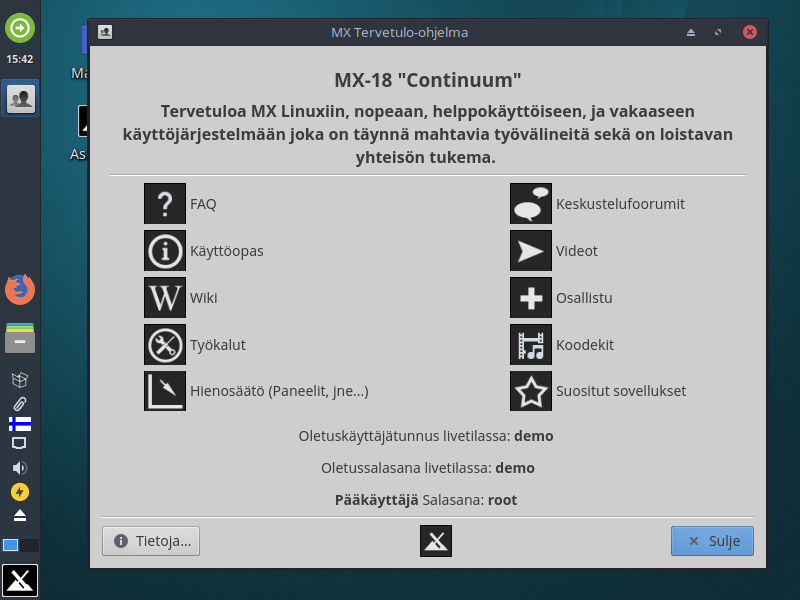
\includegraphics[width=0.9\textwidth]{asen/welcome}
        \caption{Tervetulo-ohjelma}
        \label{fig:welcome}
    \end{center}
\end{figure}

\section{Asennuksen aloittaminen}

Aloittaaksesi asennuksen, sulje kaikki muut sovellukset ikkunoiden oikeasta yläkulmasta. Paikanna asennusohjelma työpöydältä ja avaa se tuplaklikkaamalla sitä kursorilla. (Kuva \ref{fig:asenna})

\begin{figure}[htpb]
    \begin{center}
        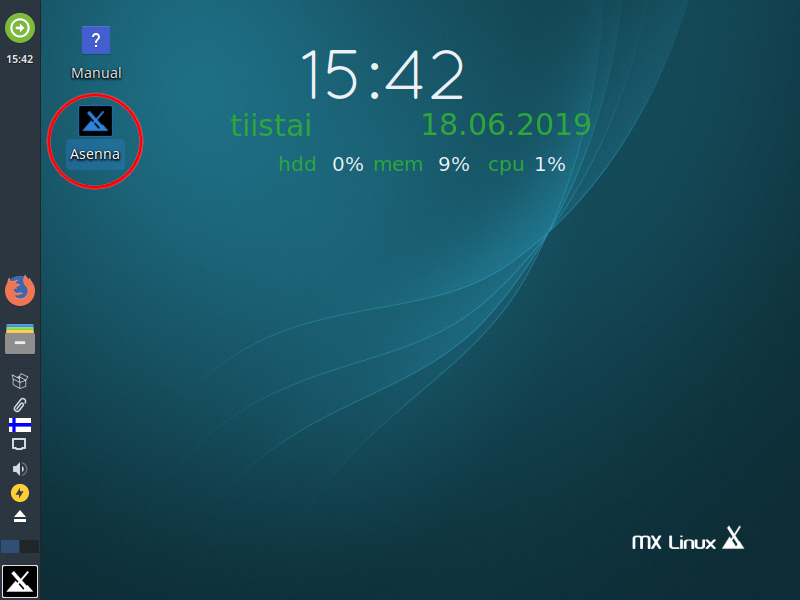
\includegraphics[width=0.875\textwidth]{asen/asenna}
        \caption{Asennusohjelman pikakuvake ympyröitynä}
        \label{fig:asenna}
    \end{center}
\end{figure}

\subsection{Asennusohjelma}

Asennusohjelma käynnistyy perinteisenä ikkunana. Tässä ikkunassa tehdään kaikki tarvittavat määritykset ja lopuksi jakelu asennetaan jakelu kovalevylle.

Ensimmäisessä vaiheessa on lyhyt esittelyteksti sekä näppäimistöasetusten valinta. Mikäli näppäimistön asettelun kohdalla ei lue \textbf{fi}, muuta asettelua painamalla \textit{Muuta näppäimistön asetuksia}. Kun näppäimistön asettelu on vaihdettu sopivaksi, asennusta voi jatkaa painamalla Seuraava-painiketta. (Kuva \ref{fig:as1})

\begin{figure}[htpb]
    \begin{center}
        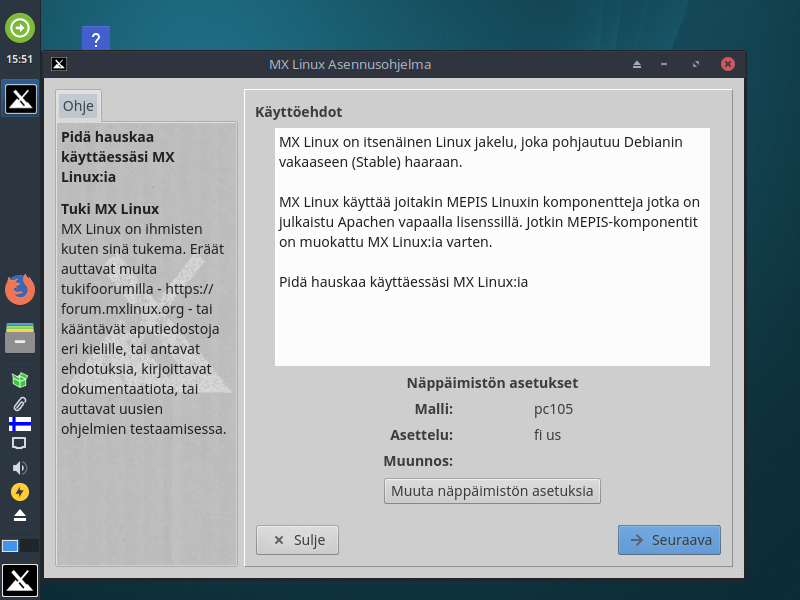
\includegraphics[width=0.875\textwidth]{asen/asennusohjelma1}
        \caption{Asennusohjelman ensimmäinen vaihe}
        \label{fig:as1}
    \end{center}
\end{figure}
\clearpage

\subsection{Osiointi}
Asennusohjelman seuraavassa vaiheessa kovalevy osioidaan. Uusille käyttäjille suositellaan valitsemaan automaattinen osointi valitsemalla kuvassa näkyvän vaihtoehdon \textit{Asenna automaattisesti käyttäen koko levyä}. Tällöin asennusohjelma osioi valitun kovalevyn automaattisesti ja käyttäjän ei tarvitse huolehtia asiasta.
Mikäli olet ennen osioinut GNU/Linux-järjestelmiä ja haluat tehdä sen manuaalisesti, valitse vaihtoehto \textit{Mukautettu asennus olemassaoleville osioille} ja siirry oppaan kohtaan \ref{sec:manual}. (Kuvat \ref{fig:osiointi} ja \ref{fig:auto})

\begin{figure}[htpb]
    \begin{center}
        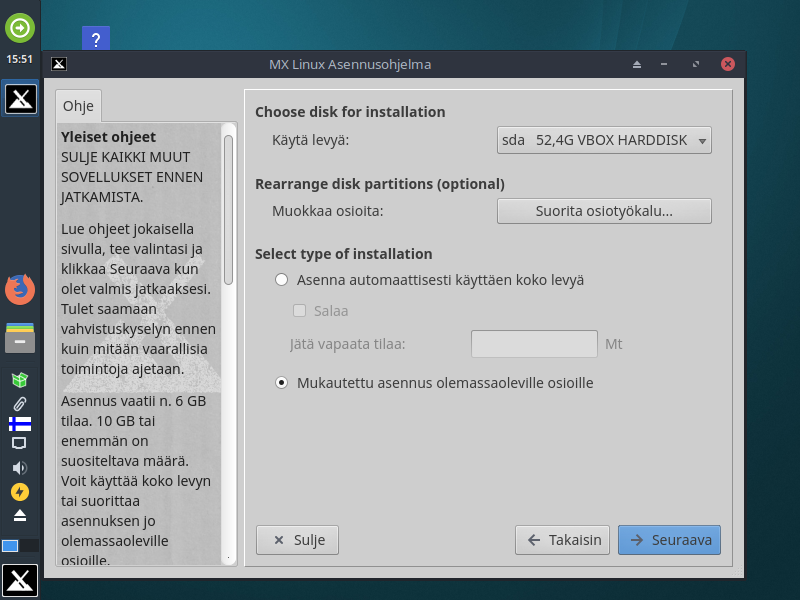
\includegraphics[width=0.7\textwidth]{asen/osiointi}
        \caption{Asennusohjelman osiointivaihe}
        \label{fig:osiointi}
    \end{center}
\end{figure}
\begin{figure}[htpb]
    \begin{center}
        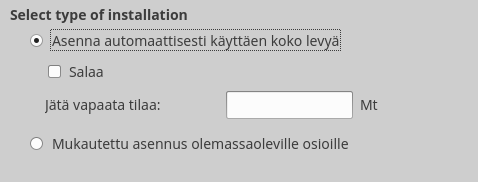
\includegraphics[width=0.65\textwidth]{asen/osiointi_auto}
        \caption{Osiointitavan valitseminen asennusohjelmassa}
        \label{fig:auto}
    \end{center}
\end{figure}


\subsubsection{Manuaalinen osiointi}
\label{sec:manual}
Manuaalista osiointia varten avaa haluamasi osiointityökalu tai suorita \textit{gparted}-työkalu painamalla \textit{Suorita osiotyökalu} -painiketta. Työkalun avauduttua, valitse yläreunasta oikea kovalevy ja poista mahdolliset aikaisemmat osiot painamalla osiota hiiren oikealla painikkeella, ja valitsemalla \textit{poista}. Kuvassa näkyy kovalevy, josta on poistettu jokainen osio, ja on täten valmis osioitavaksi MX Linux 18 -asennusta varten. (Kuva \ref{fig:varaamaton})
\clearpage
\begin{figure}[htpb]
    \begin{center}
        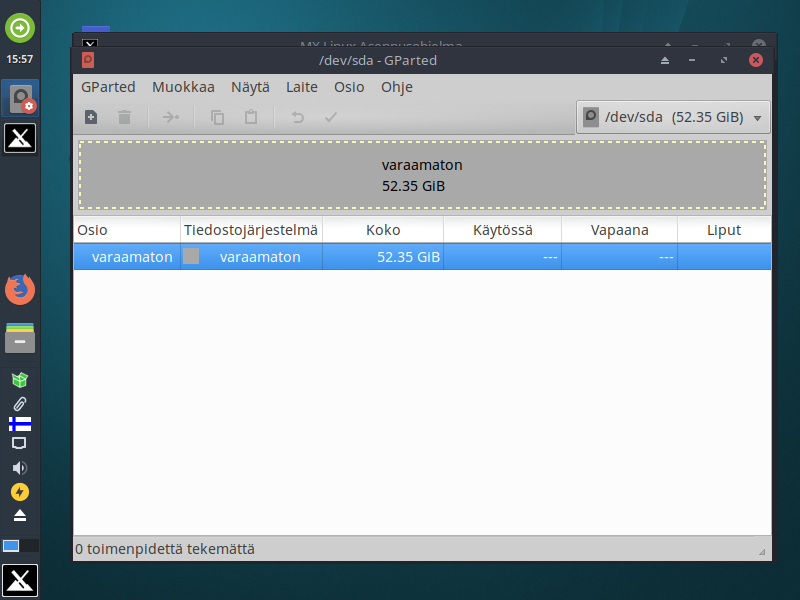
\includegraphics[width=0.98\textwidth]{asen/osiointi_gparted}
        \caption{Gparted-työkalu}
        \label{fig:varaamaton}
    \end{center}
\end{figure}
\begin{wrapfigure}{r}{0.5\textwidth}
  \begin{center}
    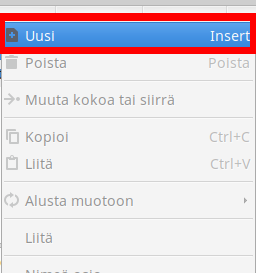
\includegraphics[width=0.35\textwidth]{asen/osiointi_gparted_uusi}
  \end{center}
  \vspace*{-3mm}
  \caption{Uuden osion luominen Gparted\\-työkalun valikosta}
  \label{fig:uusi}
\end{wrapfigure}
Aloita osiointi luomalla swap-osio. Swap tarkoitaa keskusmuistissa olevan tiedon siirtämistä massamuistille, keskusmuistitilan loppuessa. 
Swap-osio tehdään mahdollisesti siirrettävää dataa varten. MX Linux 18 suosittelee swap-osion kooksi hieman laitteiston keskusmuistia isompaa määrää. Luo osio painamalla varaamatonta aluetta hiiren oikealla painikkeella ja valitsemalla \textit{uusi}. (Kuva \ref{fig:uusi})
Valitse osion tiedostojärjestelmäksi \textit{linux-swap}.
Aseta myös osion koko. Koko syötetään kohtaan \textit{Uusi koko (MiB)}. Jos laitteessasi on esimerkiksi 8 gigatavua keskusmuistia, anna osion kooksi 8000 MiB. Tässä oppaassa jakelu asennetaan laitteistolla, jossa on kaksi gigatavua keskusmuistia, joten swap-osion koko on 2000 mebitavua eli noin 2,1 gigatavua. (Kuva \ref{fig:swap})
\clearpage
\begin{figure}[htpb]
    \begin{center}
        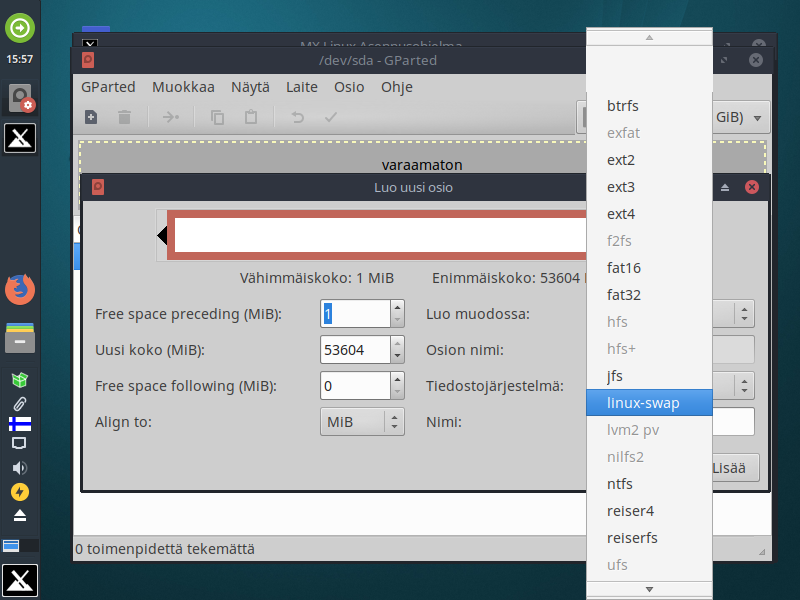
\includegraphics[width=0.7\textwidth]{asen/osiointi_gparted_swap}
        \caption{Swap-osion tiedostojärjestelmä}
        \label{fig:swap}
    \end{center}
\end{figure}



Luo seuraavaksi juuri-osio. Juuri- eli root-osioon asennetaan varsinainen käyttöjärjestelmä. Osio sisältää kaikki käyttäjän asentamat ohjelmistot ja asetukset. Valitse Gparted-työkalussa varaamaton alue ja paina \textit{Uusi}. Osiolle suositeltu tiedostojärjestelmä on ext4. Osion kooksi suositellaan koko loppu levytilaa. (Kuva \ref{fig:root})

\begin{figure}[htpb]
    \begin{center}
        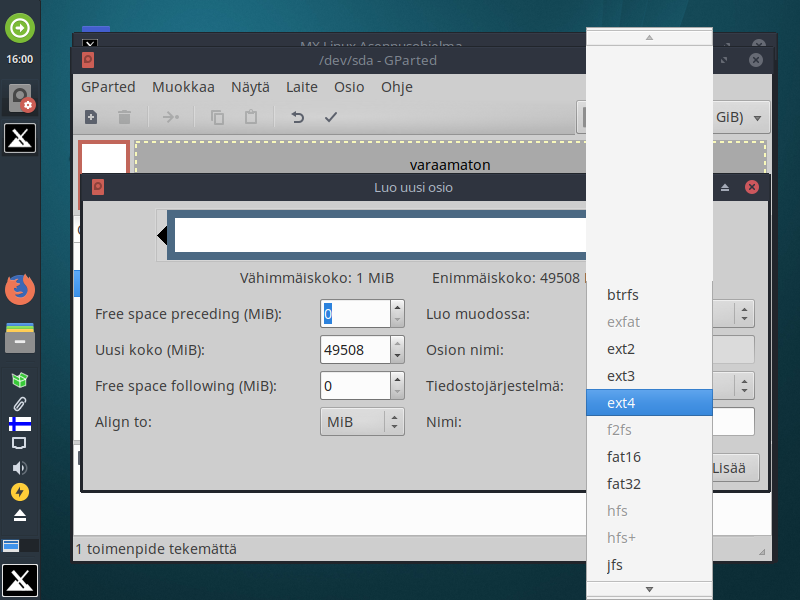
\includegraphics[width=0.7\textwidth]{asen/osiointi_gparted_root}
        \caption{Swap-osion tiedostojärjestelmä}
        \label{fig:root}
    \end{center}
\end{figure}
\section{<++>}

\end{document}

